%%%%%%%%%%%%%%%%%%%%%%% file typeinst.tex %%%%%%%%%%%%%%%%%%%%%%%%%
%
% This is the LaTeX source for the instructions to authors using
% the LaTeX document class 'llncs.cls' for contributions to
% the Lecture Notes in Computer Sciences series.
% http://www.springer.com/lncs       Springer Heidelberg 2006/05/04
%
% It may be used as a template for your own input - copy it
% to a new file with a new name and use it as the basis
% for your article.
%
% NB: the document class 'llncs' has its own and detailed documentation, see
% ftp://ftp.springer.de/data/pubftp/pub/tex/latex/llncs/latex2e/llncsdoc.pdf
%
%%%%%%%%%%%%%%%%%%%%%%%%%%%%%%%%%%%%%%%%%%%%%%%%%%%%%%%%%%%%%%%%%%%


\documentclass[runningheads,a4paper]{IEEEtran}
\usepackage{amsmath}
\usepackage{amssymb}
\setcounter{tocdepth}{3}
\usepackage{graphicx}
\usepackage{listings}
\usepackage{color}
\usepackage{scrextend}
\usepackage{caption}
\usepackage{booktabs}
\usepackage{url}
\setlength{\tabcolsep}{2pt}
\renewcommand{\arraystretch}{1.2}
\urldef{\mailsa}\path|rparundekar@gmail.com|
\newcommand{\myTitle}{Understanding `Things' using Semantic Graph Classification} 
\newcommand{\myName}{Rahul Parundekar} 

%\newcommand{\keywords}[1]{\par\addvspace\baselineskip
%\noindent\keywordname\enspace\ignorespaces#1}

\begin{document}

%\mainmatter  % start of an individual contribution

% first the title is needed
\title{\myTitle}

% a short form should be given in case it is too long for the running head
%\titlerunning{\myTitle}

% the name(s) of the author(s) follow(s) next
%
% NB: Chinese authors should write their first names(s) in front of
% their surnames. This ensures that the names appear correctly in
% the running heads and the author index.
%
\author{\myName}
%
%\authorrunning{\myName}
% (feature abused for this document to repeat the title also on left hand pages)

% the affiliations are given next; don't give your e-mail address
% unless you accept that it will be published
%\institute{
%Machine Learning Nanodegree, Udacity\\
%\mailsa\\
%\url{https://github.com/rparundekar}}

%
% NB: a more complex sample for affiliations and the mapping to the
% corresponding authors can be found in the file "llncs.dem"
% (search for the string "\mainmatter" where a contribution starts).
% "llncs.dem" accompanies the document class "llncs.cls".
%

%\toctitle{\myTitle}
%\tocauthor{\myName}
\maketitle

\begin{abstract}
The world around us contains different types of things (e.g. people, places,
objects, ideas, etc.) that are defined by their attributes and relationship. To act automatically on such data, any software Agent needs to be able to infer the meaning of these things that form a Semantic Graph. Using DBpedia as an exemplary dataset, we create a robust type inferencing system in the presence of noisy data and the Open World Assumption on the Semantic Web. Our approach extracts features from the Semantic Graph using multiple Random Walks and then performs multi-label classification using Deep Neural Networks. This report presents our exploration, experimentation, and results of identifying DBpedia ontology types, categories and Yago ontology types for individuals in DBpedia. Our method consistently performs better than state-of-the-art type inferencing systems, like SDtype and SLCN, from which we conclude that Random Walk based feature extraction and multi-label classification is a promising approach in understanding things and contexts in domains that represent information as a Semantic Graph.
%\keywords{Ontology, Semantic Web, Random Walks, Graph Classification, Deep Learning}
\end{abstract}

\section{Definition}
\subsection{Project Overview}

\subsubsection{Problem Domain}

The world around us contains different types of things (e.g. people, places,
objects, ideas, etc.). Predominantly, these things are defined by their attributes
like shape, color, etc. They are also defined by their relationships with 
other things. For example, Washington D.C. is a
place and U.S.A is a country. But they have a relationship of Washington D.C.
being the capital of U.S.A., which adds extra meaning to the city. 

Our domain for the project is the Semantic Web where information is represented with well-defined meaning, thus better enabling computers (Agents) and people to work in co-operation \cite{berners2001semantic}. It is an extension of the Knowledge Representation and Reasoning topic within Artificial Intelligence that aims at representing such things and their attributes and relationship using symbols at web-scale and enabling Agents to reason about them. 
Information in the Semantic Web is represented as Semantic Graphs, since the nodes, properties, and edges of graphs are very well suited to describe the things, their attributes,
and their relationships with other things in the domain. Semantic Graphs are also popularly used in various other domains like Linked Data~\cite{heath2011linked}, Spoken Dialog Systems \cite{socher2011parsing}, Social Networks \cite{backstrom2011supervised}, Scene Understanding~\cite{socher2011parsing}, Virtual \& Augmented Reality \cite{lugrin2007making}, etc. 
%A few other domais where such Semantic Graphs are used are:
%\begin{itemize}
%\item Linked Data - The web-scale Semantic Graph of open data~\cite{heath2011linked}.
%\item Spoken Systems - Output of NLP\footnote{https://en.wikipedia.org/wiki/Natural\_language\_processing} systems is a parse
%tree \cite{socher2011parsing}.
%\item Social Networks are also graphs \cite{backstrom2011supervised}.
%\item Scene Recognition - High level semantic information (e.g. arrangement of things) in images are Semantic Graphs \cite{socher2011parsing}.
%\item Virtual and Augmented Reality (VR and AR) environments can be represented as Semantic Graphs \cite{lugrin2007making}.
%\end{itemize}


\subsubsection{Project Origin}
In such a setting, an Agent on the Semantic Web needs to be able to understand the information that it comes across. By inferring the type of the thing, it may be able to perform automated actions. The project is motivated by 
our assumption that if an Agent is able to classify things by understanding
its attributes and relationships into semantic types, we could in the future 
generalize it to an Agent that can act on the meaning and context of the things. For example, such an Agent can be a virtual assistant  \cite{tang2017emergence} \cite{schmeil2007mara}, an autonomous system \cite{cordts2015cityscapes} or other software\cite{backstrom2011supervised}. 

%For example, the Agent applications for domains above are:
%\begin{itemize}
%\item Linked Data - Understand and automatically assist users at web-scale \cite{berners2001semantic}.
%\item Spoken Systems - Understanding user Intent by Virtual Assistants like Siri, Alexa, etc. for home automation \cite{tang2017emergence}. 
%\item Predicting and Recommending links in Social Networks \cite{backstrom2011supervised}.
%\item Scene recognition - Urban scene understanding \cite{cordts2015cityscapes}.
%\item Virtural Assistants like Mara \cite{schmeil2007mara} in VR and AR environments.
%\end{itemize}


\subsubsection{Related Datasets}
\label{dataset}
We use DBpedia\footnote{http://wiki.dbpedia.org/}  as an exemplary dataset 
as a starting point to study type inferencing in a Semantic Graph. 
DBpedia is an encyclopedic Semantic Graph of structured information extracted from Wikipedia (e.g. page links, categories, infoboxes, etc.) \cite{lehmann2015dbpedia} \cite{dbpedia-swj}. For example, in the subset of DBpedia shown in Figure~\ref{graph}, we can see the individual for United\_States (on the left) connected to Washington D.C. using the \textit{capital} relationship. 

Each \textit{thing} in DBpedia has one or more \textbf{types} and \textbf{categories} associated with it. 
The user community creating DBpedia maintains an Ontology\footnote{An Ontology is defined as a formal specification of the types, properties, and relationships of the entities that exist for a particular domain.} that specifies these types of the \textit{things}. 
We use the subset of DBpedia\footnote{http://wiki.dbpedia.org/downloads-2016-04}, which was generated from the March/April 2016 dump of Wikipedia. In this dataset, we use the \textit{things}, their attributes and 
their relationships extracted from Wikipedia infoboxes (\texttt{infobox\_properties\_en.ttl}) using and the DBpedia Ontology (\texttt{dbpedia\_2016-04.owl}). We also use the types associated with the \textit{things} (\texttt{instance\_types\_en.ttl} and \texttt{yago\_types.ttl}) and the categories (\texttt{article\_categories\_en.ttl}) they belong to. The types and categories  associated with United States and Washington D.C. can be seen in Figure~\ref{typeExamples}.

\begin{figure}[h]
\centering
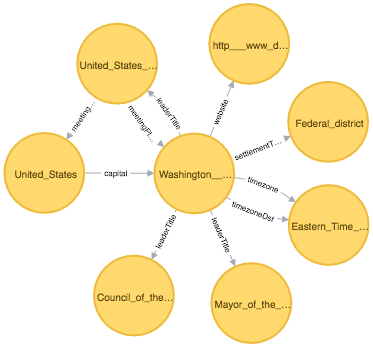
\includegraphics[width=3.25in]{figures/graph.png}
\caption{Example neighborhood of Washington D.C. in the DBpedia Semantic Graph. The United\_States individual is connected to it via the \textit{capital} relationship.}
\label{graph}.
\end{figure}

Our goal is to try and estimate the types and categories of such \textit{things} from their attributes and relationships.  
%For example, if you look at examples of categories in DBpedia, Achilies has been
%put into the categories - demigods, people of trojan war, characters in Illead, etc.
%What makes him part of those categories? Can we learn the definitions of these
%based on the attributes and relationships of Achilies? 
%
%\subsubsection{Other Approaches:}
%{\color{red} TODO: Explain the approaches briefly}

\vspace{-10pt}
\subsection{Problem Statement}
\label{problemStatement}
Traditionally, type inferencing in the Semantic Web has been done with inference engines (e.g. OWL-DL uses SHIQ description logics \cite{horrocks2003shiq} for inferences). However, as pointed out in Paulheim et. al \cite{paulheim2013type}, the actual Semantic Web data in the wild contains a lot of noise. Even a single noisy instance along with the inference rules can break the entailments in the types or can add new entailments that may be incorrect. Thus, we need a robust way of identifying the types of the things in the Semantic Web.  
In addition to the noise, the Semantic Web also makes an \textit{Open World Assumption} \cite{drummond2006open}. In the \textit{Open World Assumption}, the Agent cannot assume that some proposition (i.e. some fact in the world) is \textbf{NOT TRUE} because it is \texttt{absent}. 
%Since the Agent may not have full visibility into the data, it may think the proposition to be \texttt{false} when it actually might be \texttt{true}. In classic Machine Learning on the other hand, typically the feature is known to be \texttt{true} or \texttt{false} depending on whether it is \textbf{actually \texttt{true} or \texttt{false}} (i.e. ground truth is known). Our type classification should also consider this assumption.

\subsubsection{Problem Definition}
Given the Semantic Graph for \textit{things} in DBpedia (containing their attributes and relationships with other \textit{things}), we would like to create a classifier using Machine Learning techniques that can provide a type inferencing mechanism in the presence of noisy data and the inherent \textit{Open World Assumption} made by the Semantic Web. Multi-class classifiers are used in Machine Learning to create models to classify data into ONE of the multiple classes. However, in DBpedia, one \textit{thing} can belong to MORE THAN ONE class. To perform such classification, we need to create a Multi-label classifier~\cite{tsoumakas2006multi}\footnote{The Canadian Institute for Advanced Research's \texttt{CIFAR-100} dataset is another example where the data can have more than one classes associated with it~\cite{krizhevsky2009learning}}. There has been some work in combining random walks on graphs with Deep Learning. Perozzi et. al~\cite{perozzi2014deepwalk}, for example, use a social network graph for link prediction and recommendation.  It is not, however, a semantic graph.

\subsubsection{Outline of Tasks} We use a four-phased approach to solve the problem. 
\begin{itemize}
\item \textbf{Feature Extraction Phase:} We extract multi-label target vectors from the type and category files and also extract feature vectors from the Semantic Graph to make it Machine Learning-ready using Random Walks \cite{tsuda2010graph}. These Random Walks extract features by taking a number of walks of varying length on the Semantic Graph and noting down each attribute or relationship that we step across. 
\item \textbf{Feature Exploration Phase:} Next, we explore the type of steps available and their contribution to the classes using Logistic Regression and Fully-connected Neural Networks. 
\item \textbf{Model Experimentation Phase:} We then experiment with different walk lengths and types of data for our Random Walks, using one Fully-connected Neural Network structure that we select based on the previous phase. Once we understand the best performing step-types, lengths and number of steps for Random Walks, we proceed with the final phase.
\item \textbf{Type Inferencing Phase:} In this last phase, after refining the model, we perform the final classification by inferring the types and categories of DBpedia using multi-label classification. 
\end{itemize}

Our expected result is that the model is able to perform multi-label classification and outperform benchmarks SDtype\cite{paulheim2013type} and SLCN\cite{melo2016type} (discussed later) for type and category inference in DBpedia. 

%We classify the \textit{things} in DBpedia and identify their types and categories
%based on the semantic graph of 
%their attributes and their relationships. 
%While the dataset is a Semantic Graph, the classic algorithms in Machine Learning
%deal with feature vectors (e.g. the numerical features used to represent the object, etc.) and are aimed
%at discriminating between different inputs to those features to identify the target type/s. 
%So, in order to perform machine learning, 
%we need to extract features for the things in the graph and also create the
%target multi-label vectors to be used for training and testing. 
%
%We extract features for each thing in DBpedia 
%(hereafter called as an \textit{individual}s)
%using a Random Walk approach \cite{tsuda2010graph}. For each random walk, we start at the
%individual in the Semantic Graph. We can choose a step randomly among different kind of steps - note the attribute / relationship / incoming relationship presence and stay on same node OR note the relationship / incoming relationship name and traverse to adjacent node. The sequence of steps noted down for the walk together form the extracted feature. 
%
%By varying the length, the number of walks, and the type of steps taken, we can extract different kind of features.
%More number of walks give more number of features, which means more data to classify with. Longer length of walks result in longer sequence of steps, which means very specialized descriptions of the individual. And finally, different step types adds to the complexity of descriptions.
%
%Meanwhile, each individual
%has one or more types  associated with it. We also extract these target classes. Our target classes for each individual can come from three sources - types from the DBpedia Ontology, DBpedia categories
%and types from the Yago \cite{suchanek2007yago} Ontology (all three downloaded from the source mentioned in Section \ref{dataset} / Dataset). For each of these sources, we create multi-label target vectors dataset such that the value for the label for a type \textit{t} in the vector for each individual is \texttt{1} if the individual is an instance of type \textit{t}, or else is \texttt{0}.
%
%Once we extract the features and the target types, 
%we can then perform the Multi-label classification.  
%For each of the three sources, we vary the number of walks, length of the 
%walks and the type of the steps taken to generate the datasets and 
%then use Deep Learning to perform the Multi-label classification. 
%
%We compare the effect of varying the random walk parameters with out chosen metrics (see below) 
%and investigate some different Fully Connected Deep Neural Network
%architectures. We also compare our results with a baseline using simple Logistic Regression, 
% and also the benchmark of SDtype\cite{paulheim2013type} and SLCN\cite{melo2016type}.
%
%\subsubsection{Expected Result:}
%By comparing simple Logistic Regression and multiple Deep Learning architectures should confirm the soundness of our approach that Deep Learning approach gives more accurate results. It should also help us pick one Deep Learning architecture for the next comparison.
%
%SDtype\cite{paulheim2013type} and SLCN\cite{melo2016type} both only use incoming relationships. We compare our classification performance with these two for both DBpedia Ontology types as well as Yago Ontology types. Our hope is that the random walk features will have comparable performane to these two approaches. At the least, we expect that using the same available data as the above two approaches, our Deep Learning architecture produces better results.

\subsubsection{Metrics}
The \texttt{$F_1$-score}  is the harmonic mean of the \texttt{precision} and the \texttt{recall} of a model's classifications\footnote{https://en.wikipedia.org/wiki/F1\_score}. 
%
%\[F_1 = \frac{2 \cdot precision \cdot recall}{precision + recall}\]
%
%where, \texttt{precision} is the ratio of textit{true positive classifications} to the \textit{predicted positive classifications} (i.e. \textit{true positives} + \textit{false positive} classifications) and \texttt{recall} is the ratio of \textit{true positive classifications} to the \textit{possible positive classifications} (i.e. \textit{true positives} + \textit{false negative} classifications). Compared to the \texttt{accuracy} metric, which is the ratio of \textit{correct classifications} to \textit{total classifications}, the $F_1$-score is a more robust mettric for model performance since it penalizes the model more heavily for both \textit{false positive} as well as \textit{false negative} classifications.
%
We have two main reasons for choosing  $F_1$-score as our metric. First, since we have a large dataset with relatively few multi-labels class types, the presence of the labels is sparse. Because of this, the number of \textit{true negatives} will overpower the calculation of the \texttt{accuracy} score, as they will dwarf the number of \textit{false positives} and \textit{false negatives}. Second, both SDtype \cite{paulheim2013type} and SLCN \cite{melo2016type} use the $F_1$-score metric, the performance of our model could be easily compared.
Since we are performing Multi-label classification, we specialize our definition of the \texttt{precision} and \texttt{recall} score as follows:
% our output values will be a vector with length equal to the number of classes and having binary values with a value of 1 in position \textit{i} when the individual belongs to class $C_i$. We need to specialize our definition of the $F_1$ score for such data. Like in the SLCN\cite{melo2016type} paper, we we re-define  \texttt{precision}, \texttt{recall}, and \texttt{$F_1$-score} as $hP$, $hR$ and $hF$ as follows:

\[precision = \frac{\displaystyle\sum_{i=1}^{|C|} tp_i}{\displaystyle\sum_{i=1}^{|C|} tp_i + fp_i},       recall= \frac{\displaystyle\sum_{i=1}^{|C|} tp_i}{\displaystyle\sum_{i=1}^{|C|} tp_i + fn_i}\]


where $C$ is the number of target classes, $tp$ are the \textit{true positive}, $fp$ are the \textit{false positive} and $fn$ are the \textit{false positive} classifications. 


\section{Feature Extraction Phase}
\label{vectorGenerationAndFeatureExtraction}
We first convert our Semantic Graph data and the types associated with the individuals in the graph into feature vectors and target vectors that can be used for multi-label classification. 

\subsection{Creating Multi-label Target Vectors:}
\label{targetVector}
Our target classes for each individual can come from three sources - types from the DBpedia Ontology, DBpedia categories,
and types from the Yago \cite{suchanek2007yago} Ontology. To extract the multi-label target vectors, we first take the inner join of each of those three sources with the individuals available in the graph. We then create a multi-label target vector for each individual such that the value for the label for a type \textit{t} in the vector is \texttt{1} if the individual is an instance of type \textit{t}, or else is \texttt{0}.
Once we identify the inner-join and the multi-label vectors, we remove the individuals from the Semantic graph that do not have type information. While this step reduces the possible relationships we may encounter with individuals for which there is no type information available, it also removes spurious individuals (e.g. things generated from Wikipedia articles that have no discernable types, things in external datasets for which we do not have type data, etc.). See the algorithm in Figure~\ref{createTargetVectors} for more detail.
\begin{figure}[t]
\begin{lstlisting}[language=Python,basicstyle=\scriptsize, frame=single]
def createTargetVectors(semanticGraph, typeFile):
   types = {}
   typeIndex = {}

   for individual, type in typeFile:
      # We need to ensure that top level types are removed, 
      # since they will be true for all individuals.
      # Note: `owl:Thing' and `rdfs:Resource' are 
      # standard compact URLs for 
      # top level Semantic Web classes.
      if (type == `owl:Thing' || type==`rdfs:Resource'):
         continue
      
      # Perform left-join by checking if individual 
      # is present in semantic graph
      if (individual in semanticGraph):
         types[individual].append(type)
         if(type not in typeIndex):
           # By adding to type index here, we ensure that 
           # all individuals at least have one type
            typeIndex[type]=len(types)-1

   targetVectors = []
   for individual in semanticGraph:
      # Perform right-join by checking if 
      # individual has a type associated with it
      if (individual not in types):
         # Remove individual from graph
         # to complete inner-join
         del semanticGraph[individual]
      else:
         # Create the multi-label target vector such that
         # targetVector[type] = 1, if individual is 
         # an instance of that type; and 
         # targetVector[type] = 0, otherwise
         targetVector = [0] * len(types)
         for type in types[individual]:
             targetVector[typeIndex[type]] = 1
         targetVectors[individual].append(targetVector)

   return targetVectors
\end{lstlisting}
\caption{Algorithm for Creating the Multi-label Target Vectors}
\label{createTargetVectors}
\end{figure}

\subsection{Feature Extraction from the Semantic Graph:}
\label{featureExtraction}
We use a Random Walk approach to extract  features for each individual \cite{tsuda2010graph} in the reduced semantic graph. 
We start our walk on the individual for which the features are to be extracted. We then create a 
list of possible steps that we can take from that node from one or more different types of steps available. 
With the DBpedia semantic graph, the four type of steps available are - 
presence of an attribute, presence of an outgoing relationship, presence of an incoming relationship (for all these three, after taking the step we will land on the same node), and a step on an incoming or outgoing relationship (here, we will land on a different node with whom the node has a relationship). 
We then select one step from this list of available steps to land on the next node. We can then take the next step. 
By taking \textit{l} such steps
we form a path. 
This random walk of length \textit{l} then becomes one feature for our classification. By performing \textit{n} such random walks starting at one instance, we can extract up to \textit{n} unique features for that instance. We repeat this for each instance, to extract features for the entire dataset.
See the algorithm in Figure~\ref{extractFeatures} for more detail. 
\begin{figure}[t]
\begin{lstlisting}[language=Python,basicstyle=\scriptsize, frame=single]
def extractFeatures(semanticGraph, n, maxLength, stepTypes):
   walkIndex = {}
   walks = {}
   for individual in semanticGraph:
      # For n number of walks
      for i in range(n):
	# To choose the length, we compare 2 strategies:
	# Strategy 1: Fixed Length
	#   Here, the length is fixed to maxLength
	# Strategy 2: Variable length from 1 upto maxLength
        #   Here, the length is chosen with probability
        #       (maxLength-l+1) / (1+2+...+maxLength)
        #   This allows shorter walks to be more dominant,
        #   since longer walks lead to sparser features.
        #   For example, chooseLength(2) 
        #     returns l=1 with probability 2/3
        #     returns l=2 with probability 1/3
         l = chooseLength(maxLength)  
         walk = []
         currentNode=individual
         for step in range(l):
            availableSteps = []
            nextNodes = []
            # Create list of available steps from stepTypes
            # (Assume standard graph helper functions below)
            # 1. Attribute presence
            if (`attribute' in stepTypes):
              for attr,value in currentNode.attributes():
               if((`hasAttr_' + attr) not in availableSteps):
                  availableSteps.append(`hasAttr_' + attr)
                  nextNode.append(currentNode)
            # 2. Relationship presence
            if (`relationship' in stepTypes):
              for rel, node in currentNode.links():
               if((`hasRel_' + rel) not in availableSteps):
                 availableSteps.append(`hasRel_' + rel)
                 nextNode.append(currentNode)
            # 3. Incoming relationship presence
            if (`incoming' in stepTypes):
              for rel, node in currentNode.incomingLinks():
               if((`hasInRel_' + rel) not in availableSteps):
                 availableSteps.append(`hasInRel_' + rel)
                 nextNode.append(currentNode)
            # 4. Relationship step 
            # If l=1, then this is same as 2 and 3, 
            # and so we add these only if l>1
            if (`step' in stepTypes && l>1):
               for rel, node in currentNode.links():
                  availableSteps.append(rel + `->')
                  nextNode.append(node)
               for rel, node in currentNode.incomingLinks():
                  availableSteps.append (rel + `<-')
                  nextNode.append(node)
           # Take a step randomly
           stepIndex = randInt(0,len(availableSteps)-1)
           step = availableSteps[stepIndex]
           nextNode = nextNodes[stepIndex] 
           walk.append(step) #Append to the walk
           currentNode = nextNode #Move to next node
       #Add to the walks
       if walk not in walks:
           walks.append(walk) 
   return walks
\end{lstlisting}
\caption{Algorithm for Extracting Features Using Random Walks}
\label{extractFeatures}
\end{figure}

We take some additional precautions in preparing the data. We make sure that the walks are not empty. This can happen if there are no attributes or relationships extracted for the individual from Wikipedia. Individuals, where no walks were found, are also removed. Also, since the next node after taking the the attribute, relationship and incoming relationship steps is the same node, it may introduce multiple features with the same steps but different orders. To eliminate this issue, we sort the steps taken at the same node in a lexicographic order before adding their sequence to the walk.
 
\textbf{Important Note on Open vs. Closed World Assumption}
It is important to note that the meaning of the feature values, which are either \texttt{0} or \texttt{1}, here is different than classic Machine Learning. In classic Machine Learning, the feature value is \texttt{0} if the feature is absent or \texttt{1} if it is present. With the Random Walk method, however, the meaning changes. The feature is \texttt{1} if the random walk was \texttt{detected}, but the feature may be \texttt{0}, even if the feature is present but not detected. 
%We feel this nuance, which is similar to making an \textit{Open World Assumption}, is an important distinction to classic Machine Learning, which makes a \textit{Closed World Assumption}. Fortunately, this is not too bad, since by default the Semantic Web makes an Open World Assumption. 
%Another thing to note here is that even if we ask our algorithm to return \texttt{n} number of walks, if some of the walks are traversed multiple times, then the total number of features extracted may not be \texttt{n}.

\section{Analysis}
%After extracting the feature vectors and the target vectors , we performed analysis to explore the data, identify the algorithms to create the classifier, and highlight the benchmark/s against which we will compare the performance of our classifier.

\subsection{Data Exploration}
\subsubsection{Data Source}
As mentioned earlier, the source of our data is a subset of DBpedia\footnote{http://wiki.dbpedia.org/downloads-2016-04}, which was generated from the March/April 2016 dump of Wikipedia. While the data is available for multiple languages (English, French, German, etc.) and multiple RDF formats (Turtle, N-Triples, etc.)\footnote{https://en.wikipedia.org/wiki/Resource\_Description\_Framework\#Serialization\_formats}, we restricted ourselves to the English dumps in the N-Triple format. The subset of data we used can be described as two parts:

\begin{itemize}
  \item \textbf{The properties file:} The main semantic data  (attributes and relationships) that we use for our Semantic Graph are the facts extracted from Infoboxes in Wikipedia. We use the \texttt{infobox\_properties\_en.ttl} file as the source for this data. 
  \item \textbf{The type files:} Our target classes for each individual can come from three sources - types from the DBpedia Ontology, DBpedia categories, and types from the Yago Ontology. At the end of our paper, we present the performance of our algorithm for each of these sources. The source files used for these sources are \texttt{instance\_types\_en.ttl}, \texttt{article\_categories\_en.ttl} and \texttt{yago\_types.ttl}, respectively. We also use the DBpedia ontology (\texttt{dbpedia\_2016-04.owl}) to infer the parent types for those in \texttt{instance\_types\_en.ttl}.
\end{itemize}
The original number of facts in each of these sources are shown in Table~\ref{tab:sources}.
\begin{table}
\caption{Number of facts}
\begin{center}
  \begin{tabular}{ | c | c | }
    \hline
    \textbf{Source file} & \textbf{Number of facts (\#triples}) \\
    \hline
    \texttt{infobox\_properties\_en.ttl} & 30,024,094 \\
    \hline
    \texttt{instance\_types\_en.ttl} & 5,214,242 \\
    \hline
    \texttt{article\_categories\_en.ttl} & 22,583,312 \\
    \hline
    \texttt{yago\_types.ttl} & 57,879,000 \\
    \hline
  \end{tabular}
\end{center}
\label{tab:sources}.
\end{table}

\subsubsection{Reduced Semantic Graphs After Creating Target Vectors}
As explained in the algorithm in Section~\ref{targetVector}, we take the inner-join of the type data and the semantic graph to reduce the number of instances and remove unnecessary individuals without types. For the three type sources and the properties file, we have three reduced Semantic Graphs - \texttt{DBpedia-OntologyTypes}, \texttt{DBpedia-Categories}, \texttt{DBpedia-YagoTypes}. The statistics about these are described in Table~\ref{tab:graphStats1}\footnote{We limited classes to only those with a support of at least 200 individuals for DBpedia-Categories and Dbpedia-YagoTypes as explained in Section~\ref{refinement}}.
\begin{table} [h]
\centering
\caption{Total Number of Individuals and Average Number of Attributes, Relationships and Incoming Relationships}.
\label{tab:graphStats1}
  \begin{tabular}{ | c | c | c | c | c | c | }
    \hline
    \textbf{Semantic Graph} & \textbf{\# indi-} & \textbf{Avg.} & \textbf{Avg. inc.}& \textbf{Avg. \#} & \textbf{\# Types /}\\
    & \textbf{vidu-} & \textbf{\# attri-\-} & \textbf{\#relation-\-}& \textbf{relatio-} & \textbf{Categories}\\
    & \textbf{als} & \textbf{butes} & \textbf{ships} &  \textbf{nships} &\\
    \hline
    \textbf{DBpedia-OntologyTypes} & 3.18M & 5.78 & 3.58 & 2.74 & 526 \\
    \hline
    \textbf{DBpedia-Categories} & 2.26M & 6.25 & 2.89 & 2.11 &  10999 \\
    \hline
    \textbf{DBpedia-YagoTypes} & 2.78M & 5.97 & 4.21 & 3.08 &  2083\\
    \hline
  \end{tabular}
\end{table}

Figure~\ref{typeExamples} shows the example types for select individuals in the \texttt{DBpedia-OntologyTypes} dataset.
\begin{figure}[t]
\begin{lstlisting}[language=Python,basicstyle=\tiny, frame=single]
Examples Types for United_States: 
		Settlement
		Country
		PopulatedPlace

Examples for Washington__D_C_: 
		Place
		Settlement
		Location
		http___schema_org_Place

Examples for Aristotle: 
		Philosopher
		Person
		http___xmlns_com_foaf_0_1_Person
\end{lstlisting}
\caption{Examples of Types in the \texttt{DBpedia-OntologyType} Dataset}
\label{typeExamples}
\end{figure}
%\begin{table}[h]
%\centering
%\caption{Average Number of Distinct Attributes, Relationships and Incoming Relationships}
%\label{tab:graphStats2}.
%  \begin{tabular}{ | c | c | c | c | }
%    \hline
%    \textbf{Semantic Graph}  & \textbf{Average} & \textbf{Average}& \textbf{Average}\\
%     & \textbf{\# attri-\-} & \textbf{\#relation-\-}& \textbf{\# incoming}\\
%     & \textbf{butes} & \textbf{ships} &  \textbf{relationships} \\
%    \hline
%    \texttt{DBpedia-OntologyTypes}  & 4.85 & 2.30 & 0.425 \\
%    \hline
%    \texttt{DBpedia-Categories} & 5.17 & 2.18 & 0.43 \\
%    \hline
%    \texttt{DBpedia-YagoTypes} & 4.98 & 2.74 & 0.47 \\
%    \hline
%  \end{tabular}
%\end{table}

%\subsubsection{Traing and Testing Dataset from Extracted Features and Target Vectors}
%From the above reduced Semantic Graphs, we then use the algorithm described in Section~\ref{featureExtraction} to extract features for classification. We create various training and testing datasets to explore the capability of our approach. We do not describe these datasets here, and instead choose to describe them in the next section and present their statistics as we come across them in the following sections.  
%
The datasets were split into batches of upto 5000 individuals in each (lesser, if unnecessary individuals were removed). The batches were split into 80\% training - 20\% testing split\footnote{Since this is an exploratory paper and first of its kind, the real world applications are not yet clear for these datasets and comparisons are not available. Accordingly, use of separate validation and final test datasets was avoided}.  

\subsection{Algorithms and Techniques}
\label{algorithms}
%To perform the Multi-label classification, we use a Fully-Connected Neural Network. The features extracted form the input and the target vectors form the multi-label outputs such that one or more of them can be on at one time. We use Deep Learning to train and test the classifier. 
%
%We use a three phase approach: 
After the Feature Extraction Phase, we proceed with the Feature Exploration, Model Experimentation, and Type Inference phases. 
\subsubsection{Feature Exploration Phase} 
\label{featureExplorationPhase}
In performing our random walk, we have four types of steps we can take from any individual:
  \begin{itemize}
     \item \textbf{Attribute presence:} where we pick randomly among the attributes present, note the attribute name, and stay on the same node (see Figure~\ref{attrExamples} for examples).
\begin{figure}[t]
\begin{lstlisting}[language=Python,basicstyle=\tiny, frame=single]
Examples for United_States: 
	Features: (upto 5 of 15)
		has_imageFlag
		has_ethnicGroups
		has_populationEstimate
		has_commonName
		has_nationalAnthem

Examples for Washington__D_C_: 
	Features: (upto 5 of 17)
		has_elevationMinFt
		has_populationRank
		has_areaCode
		has_populationMetro
		has_areaWaterSqMi

Example for Aristotle: 
	Features: (upto 5 of 4)
		has_name
		has_mainInterests
		has_birthDate
		has_deathDate
\end{lstlisting}
\caption{Examples of Features of Attribute Presence Step-Type}
\label{attrExamples}
\end{figure}

     \item \textbf{Relationship presence:} where we pick randomly among the relationships present,  note the relationship name,  and stay on the same node (see Figure~\ref{relExamples} for examples).
\begin{figure}[t]
\begin{lstlisting}[language=Python,basicstyle=\tiny, frame=single]
Examples for United_States: 
	Features: (upto 5 of 4)
		hasRel_demonym
		hasRel_capital
		hasRel_largestCity
		hasRel_leaderName

Examples for Washington__D_C_: 
	Features: (upto 5 of 1)
		hasRel_leaderTitle

Examples for Aristotle: 
	Features: (upto 5 of 2)
		hasRel_influences
		hasRel_deathDate
\end{lstlisting}
\caption{Examples of Features of Relationship Presence Step-Type}
\label{relExamples}
\end{figure}

     \item \textbf{Incoming Relationship presence:} where we pick randomly among the incoming relationships present, note the incoming relationship name,  and stay on the same node (see Figure~\ref{inRelExamples} for examples).
\begin{figure}[t]
\begin{lstlisting}[language=Python,basicstyle=\tiny, frame=single]
Examples for United_States: 
	Features: (upto 5 of 153)
		hasInRel_almaMater
		hasInRel_channel
		hasInRel_hometown
		hasInRel_based
		hasInRel_label

Examples for Washington__D_C_: 
	Features: (upto 5 of 64)
		hasInRel_regions
		hasInRel_unit
		hasInRel_origin
		hasInRel_restingPlace
		hasInRel_recorded

Examples for Aristotle: 
	Features: (upto 5 of 3)
		hasInRel_influenced
		hasInRel_influences
		hasInRel_mainInterests
\end{lstlisting}
\caption{Examples of Features of Incoming Relationship Presence Step-Type}
\label{inRelExamples}
\end{figure}

     \item \textbf{Relationship Step:} where we pick randomly among the incoming and outgoing relationships and move to the node that the relationship connects our individual to. 
  \end{itemize}



For this exploration, we use only the \texttt{DBpedia-OntologyTypes} dataset. By understanding the effect of the features and their effect on different Fully-connected Neural Network structures, we can select one network structure and select the parameters of random walks in the next phase. 

We use three Fully-connected Neural Network structures for exploration. For all three, the number of inputs in the input layer equals the number of features and the number of neurons in the output layer equal the target variable. Upon experimentation, the fully connected layers were initialized using Xavier initialization (i.e. Glorot Normal initialization \cite{glorot2010understanding}), as it lets the signal reach deeper into the network since the weights are not too small or too large to start in dead or saturated regions. Based on some preliminary exploration we trained each for 5 epochs as the $F_1$-score plateaus after that, or in the case of the 8 layer network, starts overfitting. For learning, we use Adam optimizer with the Nestrov accelerated gradient approach \cite{dozat2015incorporating} (Nadam) since it is an adaptive gradient method and our data is sparse. We use `binary cross-entropy' loss function for learning. 

Except for the Simple Logistic Regression classifier, we have the following additional structure features. We use both Nadam optimizer and Batch Normalization allows for accelerated learning. To avoid overfitting, especially since the data is sparse and the network may learn very specialized definitions, we use a Dropout layer. The dropout rate was selected as 0.2 after multiple experimentations showed that rate of 0.4 was too slow, and given the large data (about 3 Million samples). Other hyper-parameters (e.g. learning rate) were kept to default values in Keras \cite{chollet2015keras}.

  \begin{itemize}
     \item \textbf{Logistic Regression:} The simple logistic regression network has only one fully-connected layer. This will help us establish a baseline with respect to the other two structures and provide us a sanity check. Figure~\ref{logistic} shows the simple network architecture.
\begin{figure}[h]
\centering
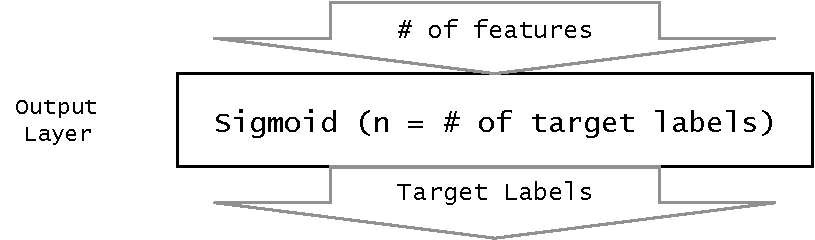
\includegraphics[width=2.25in]{figures/logistic.pdf}
\caption{Simple Logistic Regression Network Structure}
\label{logistic}.
\end{figure}

     \item \textbf{4 Layer Fully Connected Neural Network:} The first deep fully-connected neural network contains 4 layers including the input and output. The shape and sizes of the layers can be seen in Figure~\ref{full4}.
\begin{figure}[h]
\centering
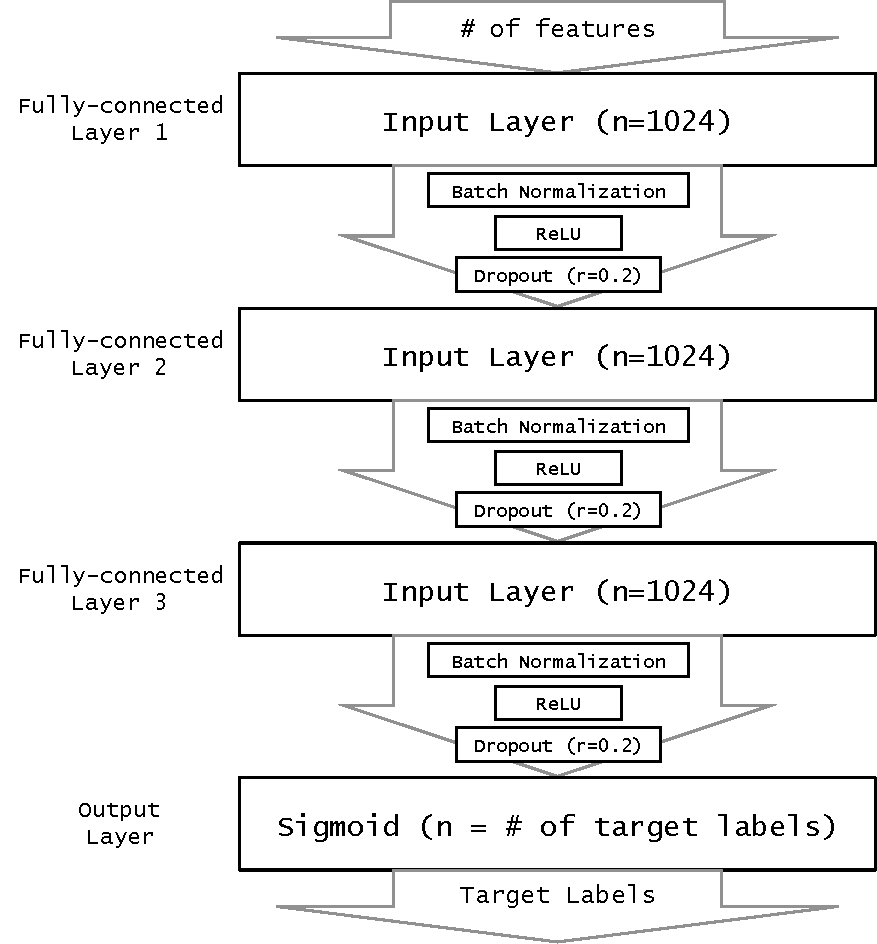
\includegraphics[width=2.25in]{figures/full4.pdf}
\caption{4 Layer Deep Neural Network Structure}
\label{full4}.
\end{figure}

     \item \textbf{8 Layer Fully Connected Neural Network} The second deep fully-connected neural network contains 8 layers including the input and output. Compared to the 4 layer network, we chose to explore another structure with fewer neurons per layer but deeper strucutre. The shape and sizes of the layers can be seen in Figure~\ref{full8}.

\begin{figure}[h]
\centering
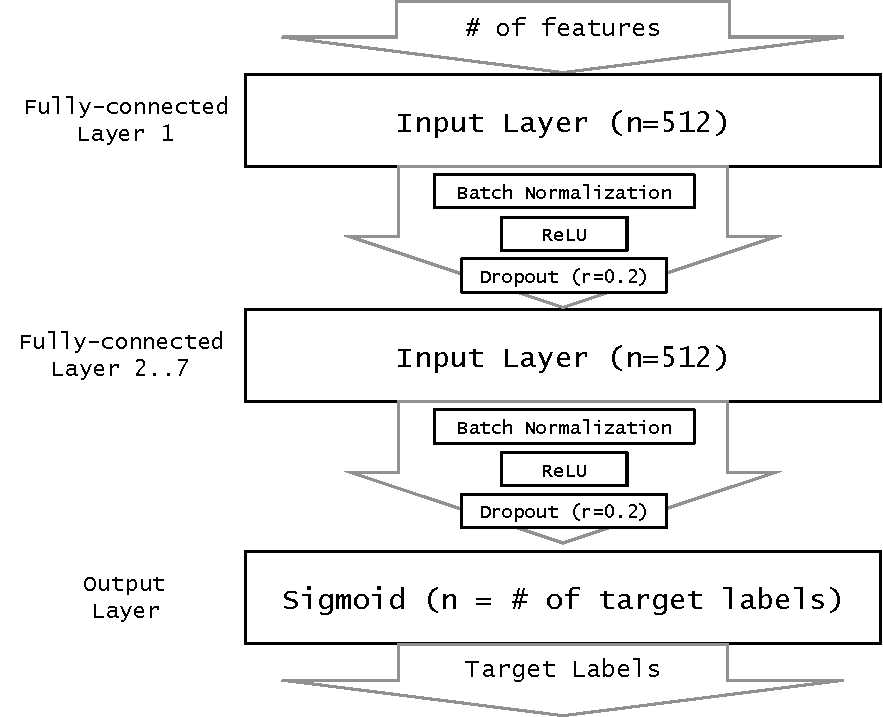
\includegraphics[width=2.25in]{figures/full8.pdf}
\caption{8 Layer Deep Neural Network Structure}
\label{full8}.
\end{figure}
  \end{itemize}

Our exploration of the feature space available is described in detail in Section~\ref{phase1}. Based on the conclusion of these exploration experiments, we select one network structure for the next phase.

\subsubsection{Model Experimentation Phase} 
We choose the Fully-connected Neural Network architecture with 4 Layers as our starting point for this phase, based on the conclusion of the previous phase (see Section~\ref{phase1}). We tried out diffferent improvements before settling down on the structure shown in Figure~\ref{full6}.
\begin{itemize}
\item We increased the depth as much as we could, but noticed that after 6 layers the network starts overfitting the data. We concluded this based on the divergence between the training and testing $F_1$-score after initial simultaneous increase. 
\item We tried layers with 2048 neurons as well. However, we noted that as we start random walks of length longer than one step, our number of features grows very rapidly and even goes into millions. With feature vectors of that length, given the memory of the GPU (4GB), we restricted to 1024 neurons to not run into memory overflow.
\item We also tried running our experiments for 10 epochs. However, we noticed little to no improvement for most of the experiments, and the training time for the larger datasets was too prohibitive to run for 10 epochs. Based on this, we restrcted to using 5 epochs. 
\end{itemize}

\begin{figure}[h]
\centering
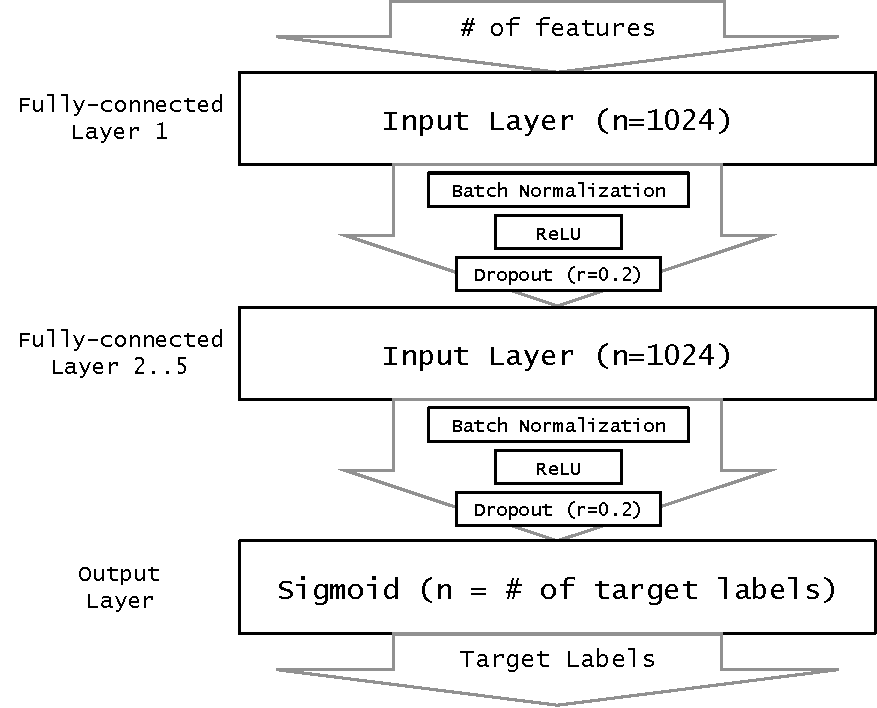
\includegraphics[width=2.25in]{figures/full6.pdf}
\caption{6 Layer Deep Neural Network Structure}
\label{full6}.
\end{figure}

After having selected a fully-connected Neural Network structure, we vary the different parameters to the \texttt{extractFeatures} function with different lengths, different number of walks and different types of steps. By comparing the classification performance of the different experiments, we can select the most appropriate parameters. For these experiments, we use only the \texttt{DBpedia-OntologyTypes} dataset. Here, we group the types of steps into two:
  \begin{itemize}
     \item \textbf{Step but stay on same node:} Steps of type attribute presence, relationship presence and incoming relationship presence.
     \item \textbf{Step and move across the relationship:} Step over any incoming and outgoing relationship and move to the next node. 
  \end{itemize}  
The delails of the experiments and results are presented in the Section~\ref{methodology}.

\subsubsection{Type Inferencing Phase} 
Finally, after having selected the random walk parameters and the network structure, we perform the final classification for the \texttt{DBpedia-OntologyTypes}, \texttt{DBpedia-Categories} and \texttt{DBpedia-YagoTypes} datasets with some refinements to the network structure, pre-processing, etc. We describe this in Section~\ref{evaluation}.

\subsection{Exploratory Visualizations}
\label{phase1}
Our exploratory visualizations come from the feature extraction phase. We use the \texttt{extractFeatures} function to extract features of four type of steps. We select incrementing lengths of 5, 10, and 25 for our random walks and explore the ability of the 3 structures described in Section~\ref{featureExplorationPhase} to learn to classify the \texttt{DBpedia-OntologyTypes} dataset. This dataset has a total of 3.18M individuals grouped into 638 batches. There are 529 target classes.

\subsubsection{Attribute Presence} 
We select the attribute randomly from all the attributes that the individual has, and note the name of the attribute (and ignore the value) for the step. Table~\ref{tab:attr} shows the $F_1$ scores of the different structures at different lengths and different number of walks. We note that performance increases with more random walks and the structure with 4 layers performs the best. The maximum $F_1$-score we reach here is 0.8767.
%Figure~\ref{attr} shows the $F_1$ scores of the different classifiers at different lengths. In the figure, we see that as the number of walks increases, the $F_1$-score also increases confirming the learning feasibility. We can also see that the network structure with 4 fully-connected layers performs better than the Logistic regression. Compared to the structure with 8 fully-connected layers, the structure consistently edges it out, while the deeper structure tends to drop the prediction $F_1$ score, suggesting overfitting. The maximum $F_1$-score we reach here is 0.8767.

\begin{table}[h]
\centering
\caption{Performance of the 3 structures using only the \textit{attribute presence} step}
\label{tab:attr}.
  \begin{tabular}{ | c | c | c | c | c | }
    \hline
    \textbf{\# of}  & \textbf{\# disitnct} & \textbf{Logistic } & \textbf{4 Layers} & \textbf{8 Layers} \\
    \textbf{random walks} &\textbf{features} &\textbf{ Regression} & \textbf{fully connected} & \textbf{fully connected}\\
    \hline
    10 & 1993 & 0.8224 & 0.8596 & 0.8590\\
    \hline
    15 & 2006 & 0.8330 &0.8687 & 0.8683\\
    \hline
    20 & 2014 & 0.8374  & 0.8733 & 0.8727 \\
    \hline
    All & 2020 & 0.8421 & 0.8765 & 0.8767\\
    \hline
  \end{tabular}
\end{table}

\subsubsection{Relationship Presence} 
Similar to the attribute presence step-type, we also explore the classification ability of the relationship presence step-type. Table~\ref{tab:rel} shows the relevant $F_1$ scores. Here too, we note that the structure with 4 layers performs the best. The maximum $F_1$-score we reach here is 0.8058.

%\begin{figure}[h]
%\centering
%  \begin{tabular}{| c | c |}
%\hline
%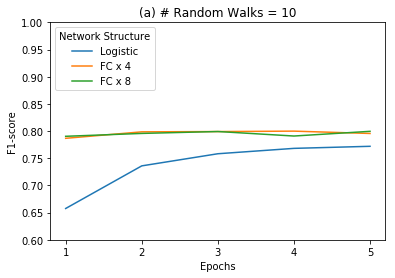
\includegraphics[width=2.25in]{figures/rel_1x10.png} & 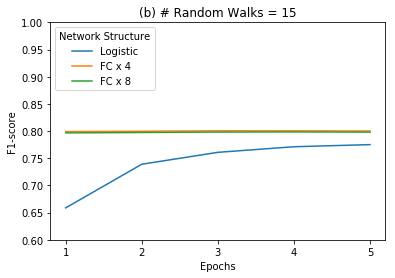
\includegraphics[width=2.25in]{figures/rel_1x15.png} \\
%\hline
%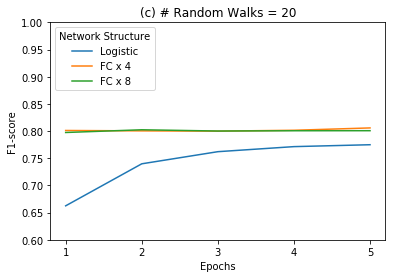
\includegraphics[width=2.25in]{figures/rel_1x20.png} & 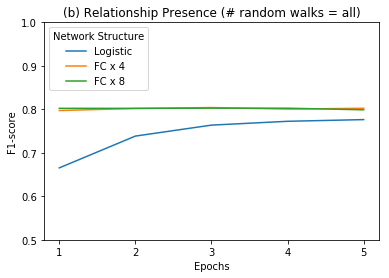
\includegraphics[width=2.25in]{figures/rel_1xall.png} \\
%\hline
%\end{tabular}
%\caption{Performance of the three neural networks with increasing number of random walks - (a) 10, (b) 15, (c) 20, (d) all using only the \textit{relationship presence} step}
%\label{rel}.
%\end{figure}

\begin{table}[h]
\centering
\caption{Performance of the 3 structures using only the \textit{relationship presence} step}
\label{tab:rel}.
  \begin{tabular}{ | c | c | c | c | c | }
    \hline
    \textbf{\# of}  & \textbf{\# disitnct} & \textbf{Logistic } & \textbf{4 Layers} & \textbf{8 Layers} \\
    \textbf{random walks} &\textbf{features} &\textbf{ Regression} & \textbf{fully connected} & \textbf{fully connected}\\
    \hline
    10 &1066 & 0.7720 & 0.7956 & 0.7995\\
    \hline
    15 & 1072& 0.7751 & 0.8001 & 0.7981\\
    \hline
    20 & 1071 & 0.7749 & 0.8058 & 0.8007\\
    \hline
    All & 1075& 0.7743& 0.8025 & 0.7989\\
    \hline
  \end{tabular}
\end{table}

\subsubsection{Incoming Relationship Presence} 
Similar to the attribute presence type of step, we also explore the classification ability of the incoming relationship presence step. Table~\ref{tab:inRel} shows the relevant $F_1$-scores. Here too, we note that the structure with 4 layers performs the best. The maximum $F_1$-score we reach here is 0.7619.

%\begin{figure}[h]
%\centering
%  \begin{tabular}{| c | c |}
%\hline
%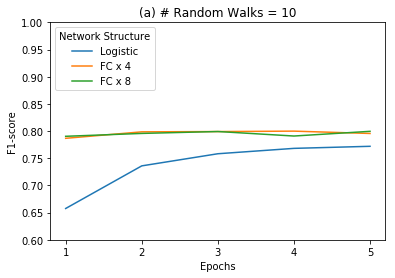
\includegraphics[width=1.6in]{figures/rel_1x10.png} & 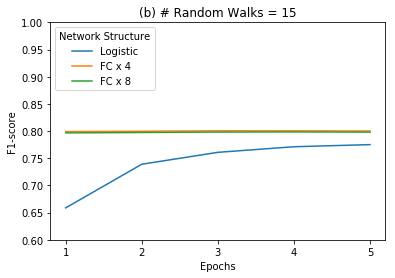
\includegraphics[width=1.6in]{figures/rel_1x15.png} \\
%\hline
%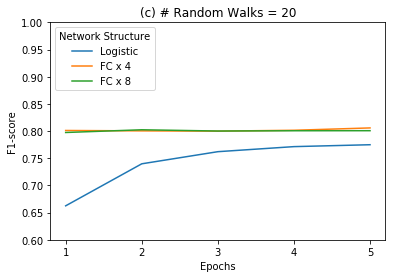
\includegraphics[width=1.6in]{figures/rel_1x20.png} & 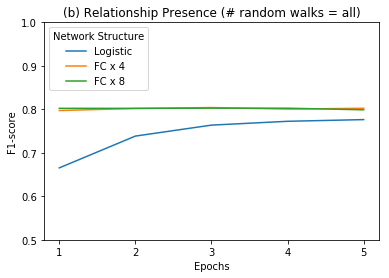
\includegraphics[width=1.6in]{figures/rel_1xall.png} \\
%\hline
%\end{tabular}
%\caption{Performance of the three neural networks with increasing number of random walks - (a) 10, (b) 15, (c) 20, (d) all using only the \textit{incoming relationship presence} step}
%\label{inRel}.
%\end{figure}

\begin{table}[h]
\centering
\caption{Performance of the 3 structures using only the \textit{incoming relationship presence} step}
\label{tab:inRel}.
  \begin{tabular}{ | c | c | c | c | c |}
    \hline
     \textbf{\# of}  & \textbf{\# disitnct} & \textbf{Logistic } & \textbf{4 Layers} & \textbf{8 Layers} \\
    \textbf{random walks} &\textbf{features} &\textbf{ Regression} & \textbf{fully connected} & \textbf{fully connected}\\
    \hline
    10 & 1043 & 0.6557& 0.7619 & 0.7612\\
    \hline
    15 & 1072 & 0.6596 & 0.7597& 0.7586\\
    \hline
    20 & 1071 & 0.6603 & 0.7563 & 0.7629\\
    \hline
    All & 1075 & 0.6693 & 0.7476 & 0.7596\\
    \hline
  \end{tabular}
\end{table}

\subsubsection{All 3} 
We also explore the classification ability of the all above three step-types. Table~\ref{tab:all3} shows the relevant $F_1$ scores. The maximum $F_1$-score we reach here is 0.9235.
\begin{table}[h]
\centering
\caption{Performance of the 3 structures using all 3 step-types}
\label{tab:all3}.
  \begin{tabular}{ | c | c | c | c | c |}
    \hline
     \textbf{\# of}  & \textbf{\# disitnct} & \textbf{Logistic } & \textbf{4 Layers} & \textbf{8 Layers} \\
    \textbf{random walks} &\textbf{features} &\textbf{ Regression} & \textbf{fully connected} & \textbf{fully connected}\\
    \hline
    10 & 4014 & 0.8256 & 0.8987 & 0.8960\\
    \hline
    15 & 4092 & 0.8428 & 0.9097& 0.9083\\
    \hline
    20 & 4110 & 0.8484 & 0.9158 & 0.9144\\
    \hline
    All & 4169 & 0.8613 & 0.9235 & 0.9219\\
    \hline
  \end{tabular}
\end{table}

Figure~\ref{1xall} below shows the comparison of the learning of the four step-types for all possible features and the three structures (we do not show the ones with fewer random walks, due to lack of space). 
\begin{figure}[h]
\centering
  \begin{tabular}{| c | c |}
\hline
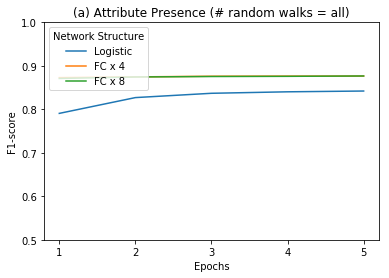
\includegraphics[width=1.6in]{figures/attr_1xall.png} & 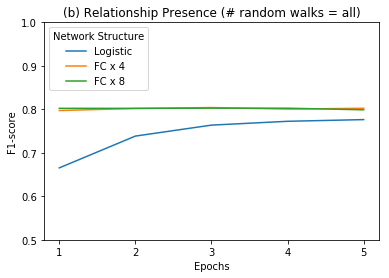
\includegraphics[width=1.6in]{figures/rel_1xall.png} \\
\hline
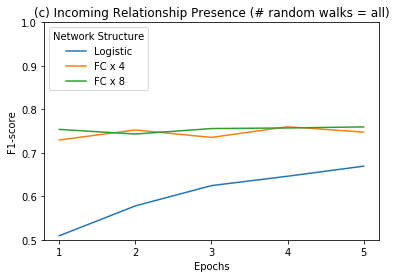
\includegraphics[width=1.6in]{figures/inRel_1xall.png} & 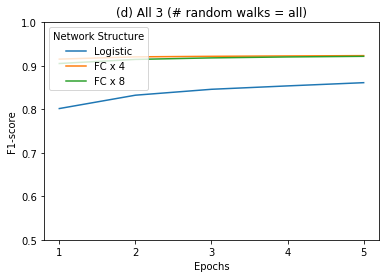
\includegraphics[width=1.6in]{figures/all3_1xall.png} \\
\hline
\end{tabular}
\caption{Performance of the 3 structures for all features for all step-types}
\label{1xall}.
\end{figure}

\subsubsection{Conclusion} From the tables and Figure~\ref{1xall}, we note that among the three types of steps, the \textit{attribute presence} step by itself has the most information to identify the classes. Meanwhile, the maximum $F_1$-score we get is 0.9235 when we use all three step-types. The \textit{incoming relationship presence} step scores the least at 0.7597. Also, among the three network structures, the Fully-connected Neural Network with 4 layers performs the best. And so we use that structure for the model experimentation phase. 

\subsection{Benchmarks}
There has been considerable prior art in inferring types of semantic data on the Semantic Web \cite{paulheim2017knowledge}\cite{miao2016automatic}.Most relevant of these are the SDtype\cite{paulheim2013type} and SLCN\cite{melo2016type}\cite{melo2017type} papers, which also try to perform type inferencing from Semantic Web data. For \texttt{DBpedia-OntologyTypes} SDtype achieves an $F_1$-score of  0.765 and SLCN\cite{melo2016type} achieves a score of 0.847. While for the \texttt{DBpedia-YagoTypes} dataset, it is 0.666 and 0.702. It should be noted that both the SDtype and SLCN papers work on the 2014 DBpedia dump, unlike ours which is the 2016 dump.

\subsubsection{Note on using attributes and relationship presence steps for classifying} 
As noted by both these papers, in original generation of DBpedia from Wikipedia, the types of the individuals were assigned using the infobox properties and the attributes and relationships were generated using a combination of that. Based on this, the authors do not use attribute presence and relationship presence for their classification as they claim the classification to be straight forward. And so, to compare with the benchmarks, we use only our algorithm with the relationship step only, having random walk length greater than 1. 

For an overall accuracy, we consider a third benchmark set by using a combination of all 3 steps of attribute, relationship, and incoming relationship presence. To generate the third benchmark, we trained the Fully-connected neural network structure with 6 layers on the dataset containing 4169 features extracted with all three step types - attribute, relationship and incoming relationship presence. With 15 epochs, to achieve maximum $F_1$ score, we set this benchmark to be 0.9254. Since the dataset is a combination of all 3 step types its performance is better than all three individually.

\section{Methodology}
\label{methodology}
In the Model Experimentation phase, we try to identify the right features to be extracted. We vary the length and number of walks, and choose from either step-types that stay on the same node or the relationship and incoming relationship step-type that moves to the adjacent node or both. We also use two strategies for selecting the length - fixed length of exactly 2 or 3, AND variable length of upto 2 or 3 with higher probability for lower lengths (as described in the \texttt{extractFeatures} function in Figure~\ref{extractFeatures}.

So in total, we have 18 variations:
\begin{itemize}
\item \textit{Length of walks} - 2 or 3
\item \textit{Number of walks} - 25, 50 or 100
\item \textit{Category of steps} - 
   \begin{itemize}
   \item \texttt{Stay:} Step but stay on same node (Attribute, relationship and incoming relationship presence) (see Figure~\ref{all3Examples} for examples), OR
\begin{figure}[t]
\begin{lstlisting}[language=Python,basicstyle=\tiny, frame=single]
Examples for United_States: 
	Features: (upto 5 of 124)
		hasInRel_production,hasInRel_regionServed
		hasInRel_citizenship,hasInRel_label
		hasInRel_twin,has_percentWater
		hasInRel_production,hasInRel_recorded
		hasInRel_origin,hasInRel_sourceLocation

Examples for Washington__D_C_: 
	Features: (upto 5 of 122)
		hasInRel_regionServed,has_areaTotalSqMi
		has_name,has_populationTotal
		hasInRel_beltwayCity,hasInRel_venue
		hasInRel_based,hasInRel_homeTown
		hasInRel_billed,hasInRel_terminusB

Examples for Aristotle: 
	Features: (upto 5 of 42)
		hasInRel_influenced,has_mainInterests
		has_deathDate,has_mainInterests
		hasInRel_mainInterests,hasRel_deathDate
		hasRel_deathDate,has_mainInterests
		hasRel_influences
\end{lstlisting}
\caption{Examples of Features of \texttt{Stay} Step Category of Walks of Length 2}
\label{all3Examples}
\end{figure} 
   \item \texttt{Move:} Step on incoming or outgoing relationship but move to adjacent node (relationship step) (see Figure~\ref{stepExamples} for examples), OR
\begin{figure}[t]
\begin{lstlisting}[language=Python,basicstyle=\tiny, frame=single]
Examples for United_States: 
	Features: (upto 5 of 105)
		office<-birthPlace->
		citizenship<-placeOfDeath->
		leaderName->predecessor<-
		regionServed<-leaderName->
		mouthCountry<-mouthLocation->

Examples for Washington__D_C_: 
	Features: (upto 5 of 83)
		leaderTitle->order<-
		stadium<-previous<-
		placeOfBirth<-director<-
		locale<-operator->
		nearestCity<-location->

Examples for Aristotle: 
	Features: (upto 5 of 20)
		influences<-author<-
		mainInterests<-placeOfBirth->
		influences<-influences->
		deathDate->birthPlace<-
		influences<-influenced<-
\end{lstlisting}
\caption{Examples of Features of \texttt{Move} Step Category of Walks of Length 2}
\label{stepExamples}
\end{figure} 
   \item \texttt{Both:} All four types of steps can be performed - attribute, relationship, and incoming relationship presence or step on an outgoing or incoming relationship. (see Figure~\ref{bothExamples} for examples), OR
\begin{figure}[t]
\begin{lstlisting}[language=Python,basicstyle=\tiny, frame=single]
Examples for United_States: 
	Features: (upto 5 of 124)
		hasInRel_institution,nationality<-
		hasInRel_production,hasInRel_restingPlace
		hasInRel_firstAired,hasInRel_releaseDate
		hasInRel_ideology,region<-
		hasInRel_manufacturer,hasInRel_subdivisionName

Examples for Washington__D_C_: 
	Features: (upto 5 of 122)
		hasInRel_governingBody,campus<-
		placeOfBirth<-birthPlace->
		hasInRel_residence,areaServed<-
		hasInRel_beltwayCity,hasInRel_city
		hasInRel_currentowner,birthDate<-

Examples for Aristotle: 
	Features: (upto 5 of 74)
		influences->has_name
		has_deathDate
		hasRel_influences,has_mainInterests
		has_deathDate,deathDate->
		hasInRel_influences,hasRel_deathDate
\end{lstlisting}
\caption{Examples of Features of \texttt{Both} Step Category of Walks of Length 2}
\label{bothExamples}
\end{figure} 
   \end{itemize} 
\item \textit{Length strategy} - Fixed or Variable length
\end{itemize}


\subsection{Preprocessing}
Since the feature extraction and target multi-label vector generation steps take care of data cleanup, and making sure that the inputs are binary, not much pre-processing was needed.
However we soon realized we quickly ran out of memory space when the magnitude of the sparsity when we take random walks. The number of features can go in the millions. Even with a modest 1024 neurons in the first layer, we quickly run out of memory. So, we encode our inputs into something reasonable. 
Since the dataset is sparse and at max, we may have 100 features in each row, we decided to superimpose features. We select an input feature size of 8384 neurons (1024x8). With this limited space, our encoding function is:
\[X[i \mod 8384]= \lfloor i \div 8384 \rfloor + 1  \]

We take additional steps to distribute the values equally in positive and negative numbers to help the network discriminate better. The absence of any random walk detected at \textit{i}th location is encoded by 0.  Since the encoding function is applied consistently to all values, we do not need any additional normalization or scaling.

\subsection{Implementation}
\label{implementation}

\subsubsection{Feature Extraction Phase}
Our feature extraction and target vector generation code was implemented in Java. Since the dataset was made available in \texttt{Turtle} RDF syntax, we used the Apache Jena Java library\footnote{https://jena.apache.org/} to parse it. Initially, we loaded the data in Neo4J Graph database\footnote{https://neo4j.com/}, since it seems the appropriate data structure. However, one complication we faced was that the creation of each random walk dataset in all phases was taking about 8-10 hours on a Macbook Pro with 16GB RAM. So we decided to optimize by holding the semantic graph in memory and performing the random walks. With this improvement, we achieved considerable speed up - we were able to create all datasets for Phase 1 and 2 in 16 hours. The target vector extraction code took about 1.5 hours on the same machine. 

\subsubsection{Feature Exploration, Model Experimentation, Type Inferencing Phases}
We use Python for the implementation of all these three phases. The Deep Learning framework used was Keras\footnote{https://keras.io/} (v1.2.2) on top of TensorFlow\footnote{https://www.tensorflow.org/} (v1.0.0). 
We developed our code in Python notebooks (one for each experiment, with common code). We created a Sequential Model for each of the network structures described before and compile them using Keras as shown in Figure~\ref{modelCode}. For each epoch, we iterated through the training batches and train the model using the \texttt{train\_on\_batch} function. After training, we test the model using the test batches. To calculate the $F_1$-score, we use our own function based on the now removed $F_1$-score metric from the Keras source code\footnote{https://github.com/fchollet/keras}. 

\begin{figure}
\begin{lstlisting}[language=Python,basicstyle=\scriptsize, frame=single]
def count_predictions(y_true, y_pred):
    true_pos = K.sum(K.round(K.clip(y_true * y_pred, 0, 1)))
    pred_pos= K.sum(K.round(K.clip(y_pred, 0, 1)))
    possible_pos = K.sum(K.round(K.clip(y_true, 0, 1)))
    return true_pos, pred_pos, possible_pos

def f1score(y_true, y_pred):
    true_pos, pred_pos, possible_pos
            = count_predictions(y_true, y_pred)
    precision = true_pos / (pred_pos + K.epsilon())
    recall = true_pos / (poss_pos + K.epsilon())
    f1score = 2.0 * precision * recall / 
                        (precision+recall+ K.epsilon())
    return f1score

#Create instance for the sequential model
deepModel = Sequential(name=`Deep Model (6 Dense Layers)')

#Add input layer
deepModel.add(Dense(1024, input_dim=dataX.shape[1],
         init=`glorot_normal'))
deepModel.add(BatchNormalization())
deepModel.add(Activation(`relu'))
deepModel.add(Dropout(0.2))

#Layer 2
deepModel.add(Dense(1024, init=`glorot_normal'))
deepModel.add(BatchNormalization())
deepModel.add(Activation(`relu'))
deepModel.add(Dropout(0.2))

#Layer 3
deepModel.add(Dense(1024, init=`glorot_normal'))
deepModel.add(BatchNormalization())
deepModel.add(Activation(`relu'))
deepModel.add(Dropout(0.2))

#Layer 4
deepModel.add(Dense(1024, init=`glorot_normal'))
deepModel.add(BatchNormalization())
deepModel.add(Activation(`relu'))
deepModel.add(Dropout(0.2))

#Layer 5
deepModel.add(Dense(1024, init=`glorot_normal'))
deepModel.add(BatchNormalization())
deepModel.add(Activation(`relu'))
deepModel.add(Dropout(0.2))

#Output layer
deepModel.add(Dense(dataY.shape[1], activation=`sigmoid', 
       init=`glorot_normal'))

#Model compilation
deepModel.compile(loss=`binary_crossentropy', 
       optimizer=`nadam', metrics=[f1score])
\end{lstlisting}
\caption{Example Sequential Model Creation for Fully-connected Strucutre with 6 Layers}
\label{modelCode}
\end{figure}

\begin{figure}
\begin{lstlisting}[language=Python,basicstyle=\scriptsize, frame=single]
#Create the train-test split
numberOfFiles = 638
testSplit=0.2
listOfFiles=list(range(1,numberOfFiles+1))
random.shuffle(listOfFiles)
splitIndex=int((1-testSplit)*numberOfFiles)

for epoch in range(0,5):
   #Train
   for index in range(0,splitIndex):
      dataX, dataY = load(xFiles[index], yFile[index])
      loss, f1score=deepModel.train_on_batch(dataX, dataY)

   #Test
   total_true_pos=0
   total_pred_pos=0
   total_poss_pos=0
   for index in range(splitIndex+1,numberOfFiles+1):
      dataX, dataY = load(xFiles[index], yFile[index])
      predY=model.predict_on_batch(dataX)
      true_pos, pred_pos, possible_pos
            = count_predictions(y_true, y_pred)
      total_true_pos+=true_pos
      total_pred_pos+=pred_pos
      total_poss_pos+=poss_pos

   #Calculate Precision, Recall and F1-score
   precision = total_true_pos /(total_pred_pos + K.epsilon())
   recall = total_true_pos / (total_poss_pos + K.epsilon())
   f1score = 2.0 * precision * recall / 
                        (precision+recall+ K.epsilon())
  print("Epoch {}: {}".format(epoch, f1score))
\end{lstlisting}
\caption{Simplified algorithm used for training and testing}
\label{trainTestCode}
\end{figure}

Another complication we faced was in the \texttt{load} function is the time taken to load the dataset from CSV files. Originally, the output of the  feature extraction and target vector generation was a pair of CSV files, one for batch. However, with the sparsity of data and a large number of features, these quickly ballooned to in order of 100s of GBs. To avoid this disk space use as well as make the loading faster we created a sparse-CSV representation, where each row would only contain the column numbers for which its value is 1. 

\subsubsection{Infrastructure}
For the feature extraction and the target vector generation Java code, we used an Apple Macbook Pro with 16GB RAM. For the Deep Learning in the other three phases we used an AWS \texttt{g2.2xlarge} instance that has one graphics card with 4GB RAM using NVIDIA GRID GPUs\footnote{https://aws.amazon.com/blogs/aws/new-g2-instance-type-with-4x-more-gpu-power/}.
Training and testing the model took about 45 minutes to 6 hours, depending on the number of features extracted in the extraction step.

\subsection{Refinement}
We first present the results of the model exploration phase. And then, we discuss the improvements we make to the structure for learning in the final type inferencing phase. 

\subsubsection{Model Experimentation Phase Results}
As described at the start of this section, we vary the length of the walks, the number of walks, the type of steps and the length strategy to conduct our experiments. Each of the following results was recorded at the end of 5 epochs (where the performance of almost all the learning plateaued). Table~\ref{tab:experiments} shows the results of the experiments. 
\begin{table}[h]
\centering
\caption{Results of Model Experimentation Phase}
\label{tab:experiments}.
  \begin{tabular}{ | c | c | c | c | c | c | c | c |}
   \hline
   \textbf{\#} & \textbf{Length} & \textbf{Step} & \textbf{Strategy}  & \multicolumn{3}{c |}{\textbf{$F_1$-score for \textit{n} steps}}\\
\cline{5-7}
   & \textbf{of walk} & \textbf{Category} & \textbf{for Length}& n=25 & n=50 & n=100\\
    \hline
   1 & 2 & \texttt{Stay} & Fixed & 0.9144 & 0.9182 & 0.9190 \\
    \hline
   2 & 2 & \texttt{Stay} & Variable  & 0.9122 & 0.9168  & 0.9177 \\
    \hline
   3 & 2 & \texttt{Move} & Fixed & 0.8401 &  0.8435 & 0.8456 \\
    \hline
   4& 2 & \texttt{Move} & Variable   & 0.8260 &  0.8328 & 0.8393 \\
    \hline
   5& 2 & \texttt{Both} & Fixed   & 0.9126 & 0.9211 & 0.9260 \\
    \hline
   6 & 2 & \texttt{Both} & Variable  &  0.9083 &  0.9137 &  0.9166\\
    \hline
   7 & 3 & \texttt{Stay} & Fixed &  0.8945 & 0.9037&  0.9102 \\
    \hline
  8 & 3 & \texttt{Stay} & Variable &  0.9015 & 0.9078 & 0.9091 \\
    \hline
  9 & 3 & \texttt{Move} & Fixed &   0.8317 & 0.8427 &  0.8509   \\
    \hline
  10& 3 & \texttt{Move} & Variable &  0.8283 & 0.8215 & 0.8299  \\
    \hline
  11& 3 & \texttt{Both} & Fixed &  0.7474 & 0.8045 &  0.8669 \\
    \hline
  12 & 3 & \texttt{Both} & Variable  &  0.8742 &  0.8785&  0.8757 \\
    \hline
  \end{tabular}
\end{table}

We can draw the following conclusions from the results in Table~\ref{tab:experiments}:
\begin{itemize}
\item \textbf{As the number of walks increases, the $F_1$-score also increases:} This is consistent with Phase 1. This is because the number of features extracted also increases. 
\item \textbf{Between fixed and variable length strategies, the fixed length works better:} When we increase the length of the walks we create more complex features. Between fixed and variable length strategies, the fixed length set is made up entirely of these complex features, while the variable length is made of simple features as well. So, given an equal number of walks the fixed strategy has more complex features and performs better.
\item \textbf{Between step categories, the one with both performs better:} With 2 steps, moving across a relationship creates new features which encode the type information of the adjacent node. So essentially, we are trying to identify the type of the node based on the type of the adjacent node. While the strategy to use attributes, relationship and incoming relationship presence works better than the strategy to move across an outgoing or incoming relationship, their combination works better than either of them. 
\item \textbf{Between features with lengths 2 and 3, a feature with length 2 performs better:} We conclude that this is because, the type of instance depends on its attributes, relationships and incoming relationships and those of its neighbors. Individuals two steps away have a lesser effect on the type of the current individual.
\end{itemize}

\subsubsection{Improvements}
\label{refinement}
Having performed optimizations for the Deep Learning network structures earlier, we do not change this itself. We had already maxed out the number of nodes we can hold in memory and depth due to overfitting concerns. We tried to optimize our network by using LeakyReLUs\cite{maas2013rectifier}, but the learning was worse. 

Upon investigating the features, we found that the step type to move across relationships had scope for improvement. We noted that sometimes, the walk returned to the original individual after traversing to another individual. We ensured that the walk did not return to the original individual. A second optimization we made was select only distinct attributes and relationships in the \texttt{stay} step category and to move only across distinct relationships in the \texttt{move} step category. By doing this, we ensure that our random walk is able to extract more diverse features about the different types of neighbors. The number of walks was also increased to 125. 

We also decided to taper the width of the network as we go deeper. Intuitively, by doing this we are forcing the network to learn feature representations in another dimension space (with fewer dimensions). One of the advantages of this in deep learning is to learn more complex representations.  Figure~\ref{final} shows the final network. Since this may require more learning, we choose 8 epochs for the training. 

\begin{figure}[h]
\centering
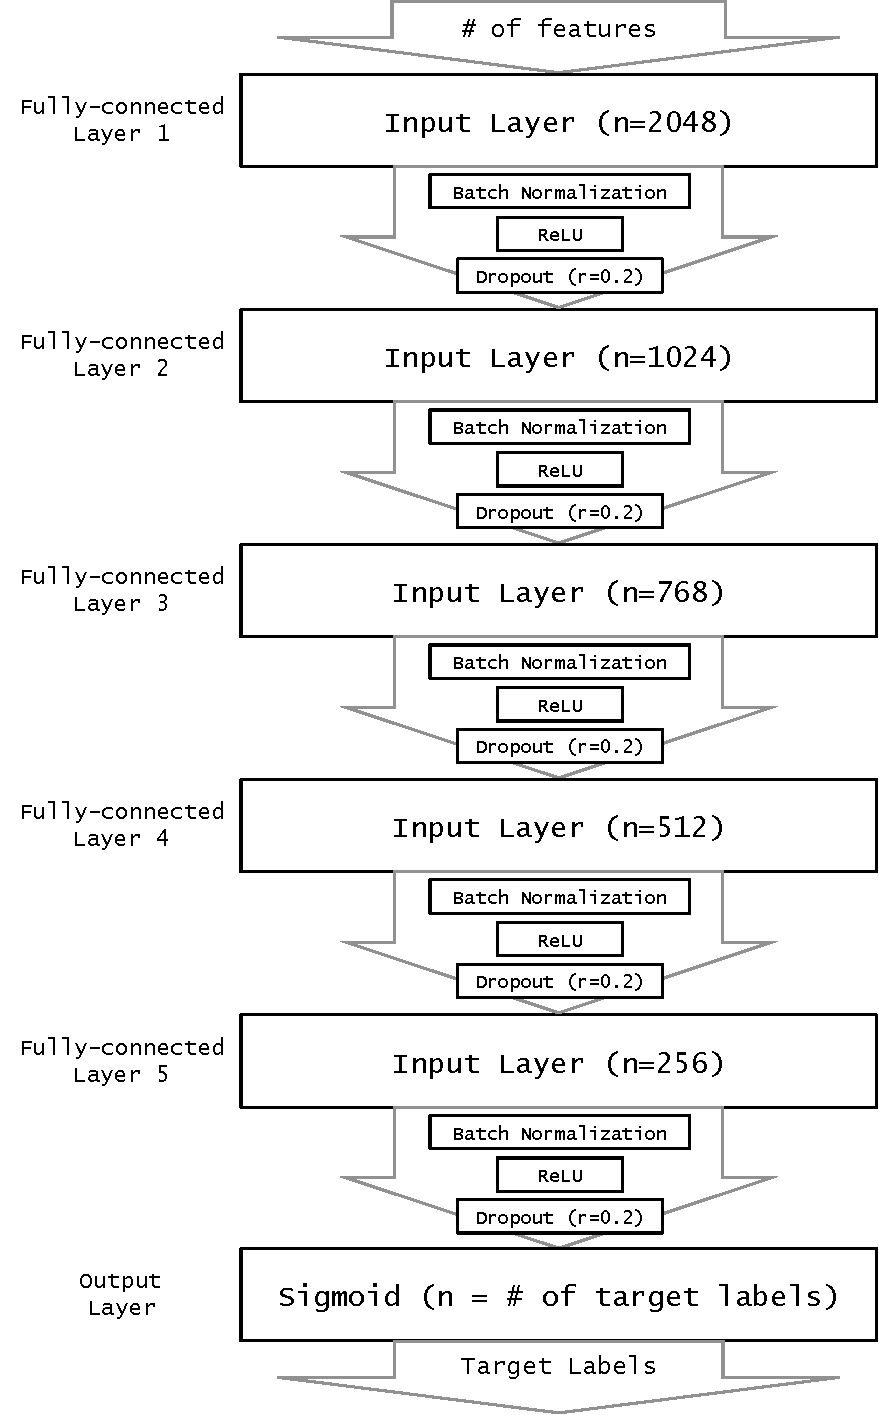
\includegraphics[width=2.25in]{figures/final.pdf}
\caption{Final Fully-connected Network Structure}
\label{final}.
\end{figure}

Our dataset was split into batches of upto 5000 individuals. While the theory behind it is not completely developved, Keskar et. al \cite{keskar2016large} suggest based on empirical observations that a small batch size, without going too small, leads to better performance due to smaller gradients. And so, instead of using the \texttt{train\_on\_batch} function in Keras, we switch to the usual \texttt{fit} function with an inner batch of length 256 from our original batch. 

We put one additional restriction on the \texttt{DBpedia-Categories} \& \texttt{DBpedia-YagoTypes} datasets. We only consider types and categories with at least 200 instance support. This was done since the long-tail of classes with fewer than 200 instance support becomes unmanageable for our classifier as the target vector would cause an out of memory error. As such, our comparison with the DBpedia-Yago benchmarks should be taken in this changed context. The final number of classes in \texttt{DBpedia-YagoTypes} was 2083 and that in \texttt{DBpedia-Categories} was 10999.

Finally, we also instead of the original train-test split, we split the dataset into training (70\%), validation (20\%) and test (10\%). We then proceed with the final Type Inferencing phase.

\section{Results}
\label{evaluation}

\subsection{Model Evaluation and Validation}
For each of the three datasets - \texttt{DBpedia-OntologyTypes}, \texttt{DBpedia-Categories} and \texttt{DBpedia-YagoTypes}, we create the training, validation and test dataset based on the refinements. The number of random walks chosen was 125. We chose the length of the walk to 2 with the fixed-length strategy. We use different step-categories as well - one where we only use the \texttt{move} step category and one using both \texttt{stay} and \texttt{move} step categories.
 Table~\ref{tab:phase3} shows the results of the experiments. 
\begin{table}[h]
\centering
\caption{Results of Type Inferencing Phase}
\label{tab:phase3}.
  \begin{tabular}{ | c | c | c | c | c |  c  | }
   \hline
   \textbf{\#} & \textbf{Dataset} & \textbf{Step} & \textbf{\# distinct}  & \multicolumn{2}{c |}{\textbf{$F_1$-score }}\\
\cline{5-6}
   &  & \textbf{Cat.} & \textbf{features}& \textbf{Validation } & \textbf{Test} \\
    \hline
   13 & \texttt{DBpedia-OntologyTypes} & \texttt{Move} & 159766 & 0.8668 & 0.8668 \\
    \hline
   14 & \texttt{DBpedia-OntologyTypes} & \texttt{Both} & 233,419 & 0.9203 & 0.9200  \\
    \hline
   15 & \texttt{DBpedia-YagoTypes} & \texttt{Move} & 167,357 & 0.8576 & 0.8594 \\
    \hline
   16 & \texttt{DBpedia-YagoTypes} & \texttt{Both} & 729,468 & 0.8550 & 0.8549  \\
    \hline
   17 & \texttt{DBpedia-Categories} & \texttt{Move} & 73,442 & 0.2909 & 0.2895   \\
    \hline
   18 & \texttt{DBpedia-Categories} & \texttt{Both} & 390,373 & 0.3388  & 0.3392  \\
    \hline
  \end{tabular}
\end{table}
Based on the results we our final model and the random walk method combined is a robust approach to performing type inferencing in noisy semantic data that also has an Open World Assumption and performs better as compared to current best benchmarks. 

\subsection{Justification}
For \texttt{DBpedia-OntologyTypes}, SDtype achieves an $F_1$-score of  0.765 and SLCN\cite{melo2016type} achieves a score of 0.847. In comparison, our model with random walks of fixed length 2 and moving to adjacent individual (i.e. using \texttt{move} step category) achieves an $F_1$ score of 0.8668. This model beaths the benchmarks. The model trained on both \texttt{move} as well as \texttt{stay} step categories achieves an $F_1$ score of 0.9200, which is on-par with our third benchmark $F_1$-score of 0.9254 set using all step-types with all available attributes, relationships and incoming relationships. This shows that features extracted with random walks of length 2 perform at least as equal to individual features. 

For the \texttt{DBpedia-YagoTypes} dataset, SDtype achieves an $F_1$-score of 0.666 and SLCN\cite{melo2016type} achieves a score of 0.702. In comparison, our model with random walks of fixed length 2 and moving to adjacent individual achieves (i.e. using \texttt{move} step category) an $F_1$ score of 0.8594. The model trained on both \texttt{move} as well as \texttt{stay} step categories achieves an $F_1$ score of 0.8549. Again, our models beat the benchmarks. However, since we remove the types with a support of less than 200 individuals, this needs further confirmation.

Our $F_1$ scores for \texttt{DBpedia-Categories} dataset models, trained on both \texttt{move} as well as \texttt{both} step categories achieves an $F_1$ score of 0.2895 and 0.3392 respectively. Since we do not have any benchmarks to compare these with, we only present these initial results.

Thus we can see that our method to extract features from Semantic Graph using  random walks and multi-label classification using deep learning better than existing best solutions that rely on incoming relationships only. It is able to perform classifications in noisy data as well as the Open World Assumption and hence is robust. Since our approach also works on an unseen test set with the same performance, we can reasonably say that the final parameters are appropriate and the model generalizes well. 


\section{Conclusion}
\subsection{Free-form Visualization}
\begin{figure}[h]
\centering
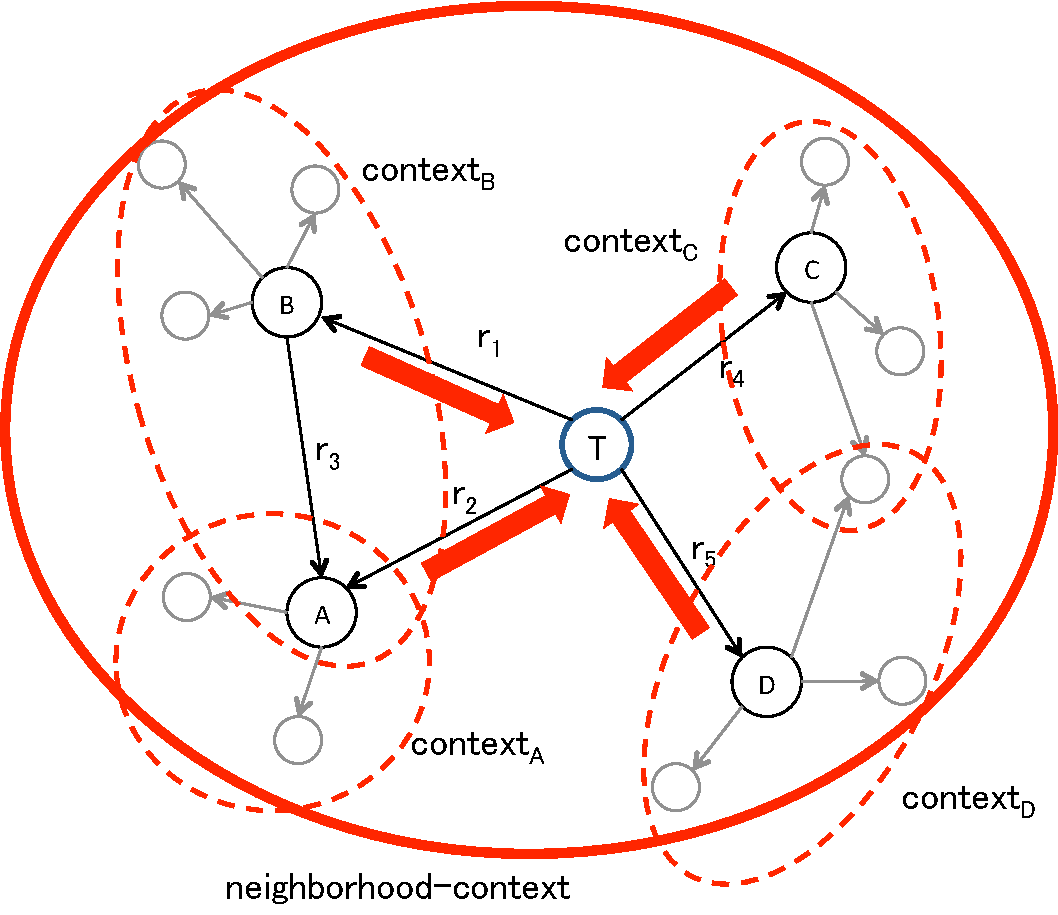
\includegraphics[width=3.25in]{figures/context.pdf}
\caption{Context encoding with Random Walks of Length 2}
\label{context}.
\end{figure}
As shown in Figure~\ref{context}, our Random Walk approach to extract features from Semantic Graphs is able to generate a neighborhood-context by encoding the contexts of the neighbors surrounding the individual we would like to classify. With a random walk of length 2, each walk encodes a signal for two types of information - the first step encodes the information of the type of the current individual based on the kind of relationships it participates in. The second information is the recursive context information about the neighboring individuals based on their neighbours. When we take multiple walks within this neighborhood, the context of the neighborhood starts adding up towards our current individual, thus helping us identify its type.

Using Deep Learning, we can create a robust classifier that uses these extracted features to identify the types in the presence of noise in the data and the Open World Assumption. Additionally, by adding the label de-noising autoencoder, we also are able to overcome noisy labels.

\subsection{Reflection}
At the onset, we set out to investigate type inferencing for individuals in a Semantic Graph by using its attributes and relationships. To do this we investigated the random walk method to extract features from the individual's neighborhood. We gradually investigated the capability of our technique to classify DBpedia individuals into multiple types in the DBpedia Ontology using the following phases: 
\begin{itemize}
\item \textbf{Feature Exploration:} We investigated different step types and their individual contribution to the classes. We also investigated different Fully-connected Neural Network structures and selected one model for further analysis.
\item \textbf{Model Experimentation:} By varying type of steps, number of walks, the length of walks, and strategy for the lengths of those walks we understood how these parameters 
\item \textbf{Type Inferencing:} Finally, after having selected one combination of parameters, we classified individuals in the \texttt{DBpedia-OntologyTypes}, \texttt{DBpedia-Categories}, and \texttt{DBpedia-YagoTypes}  datasets. 
\end{itemize}
Our results showed that this approach for classifying \textit{things} in the Semantic Graph outperform state-of-the-art inferencing techniques in the presence of noisy data and the Open World Assumption.

This end-to-end approach is both interesting in its capability as well as its novelty. While creating a sound methodology for achieving the above results was challenging and took many experiments (those that we do not report here), our results show that the random walk approach to extracting features from individuals in a Semantic Graph is a promising step to understanding the context and meaning of \textit{things}. We hope that in the future we would be able to use our approach for semantic understanding in various domains other than the Semantic Web.

\subsection{Improvements}
There are two main improvements that we feel are important to investigate in the future. 

\subsubsection{Use attribute values} 
In the current work, we completely drop the attribute values since the effective strategy to incorporate values together with the random walk strategy was not clear. By using the attributes, we feel that our approach can become better and achieve higher $F_1$-score.

\subsubsection{Noise in the labels}
We mentioned earlier that the RDF data on the Semantic Web is noisy. For this work, we assume, however, that the labels are correct. If these labels were to have noise in them as well, we would need to investigate some label de-noising techniques such as Wang et. al \cite{wang2014label}.

\subsubsection{Exploring other domains}
Finally, we would like to try our approach on other domains that use a semantic graph for inferencing like NLP, Scene Understanding, VR, and AR, etc.
\bibliography{reportBib}
\bibliographystyle{splncs}

\end{document}